We evaluated \xxx on both AWS and our cluster.

\subsection{Evaluation Setup}

talk about how we set up the evaluation

\subsection{Ease of Use}

use kad+gossip to substitute eth

\begin{figure}[ht]
  \centering
    \begin{subfigure}[b]{0.48\textwidth}
	  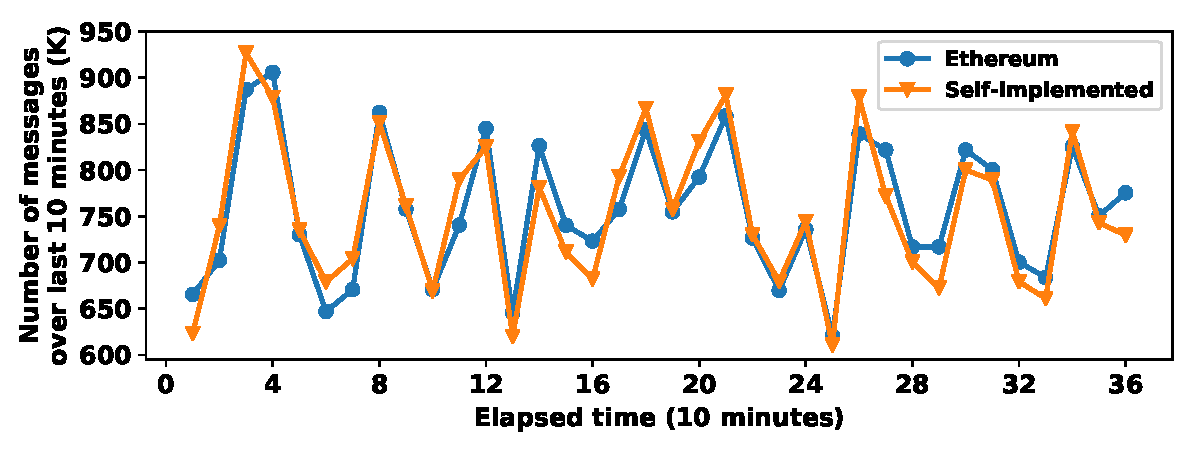
\includegraphics[width=\textwidth]{figures/eth_ourgossip_num_msg_on_time.pdf}
	  \caption{Broadcast behavior.}
	  \label{eth_ourgossip_num_msg_on_time}
    \end{subfigure}

    \begin{subfigure}[b]{0.23\textwidth}
    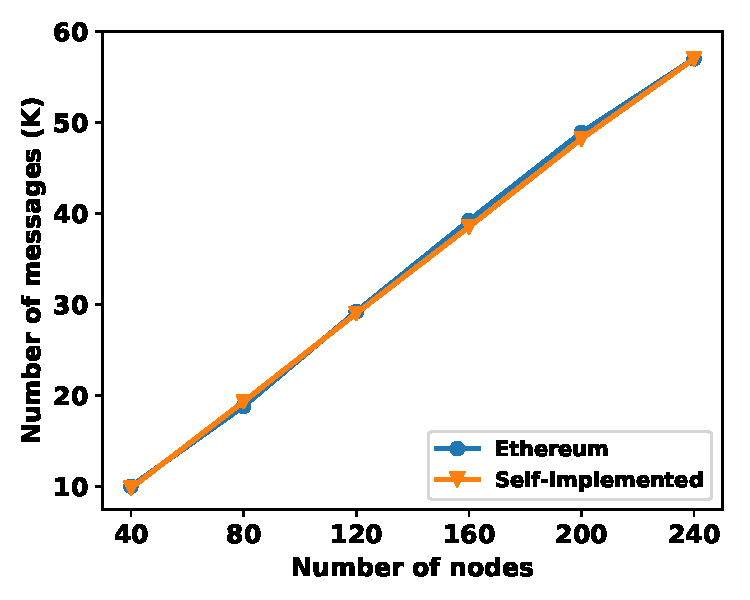
\includegraphics[width=\textwidth]{figures/eth_ourgossip_num_msg_on_num_node.pdf}
    \caption{Message complexity.}
    \label{eth_ourgossip_num_msg_on_num_node}
    \end{subfigure}
    ~
    \begin{subfigure}[b]{0.23\textwidth}
	  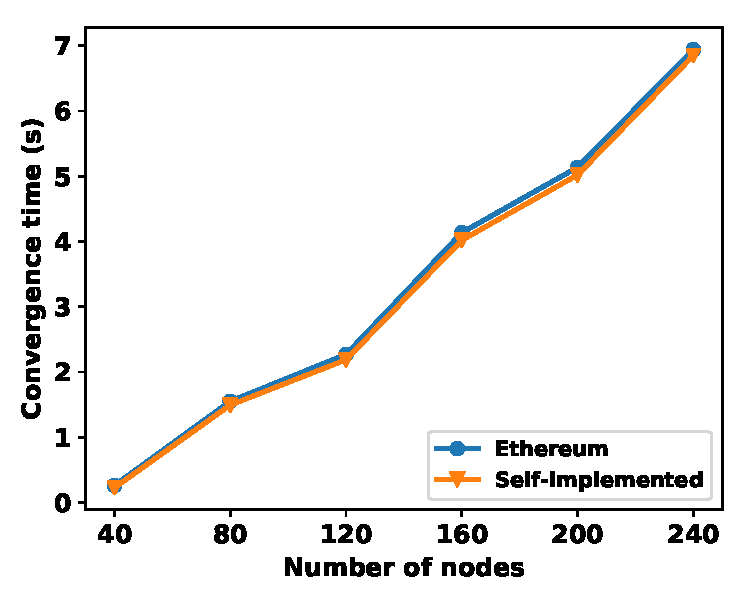
\includegraphics[width=\textwidth]{figures/eth_ourgossip_cvgtime_on_num_node.pdf}
	  \caption{Time complexity.}
    \label{eth_ourgossip_cvgtime_on_num_node}
    \end{subfigure}

	\caption{The comparison between Ethereum and self-implemented Kademlia-based Gossip.}
	\label{fig_eth_ourgossip}
	\vspace{-0.5cm}
\end{figure}

  
\subsection{Performance Improvements}

\begin{figure}[ht]
  \centering
    \begin{subfigure}[b]{0.23\textwidth}
    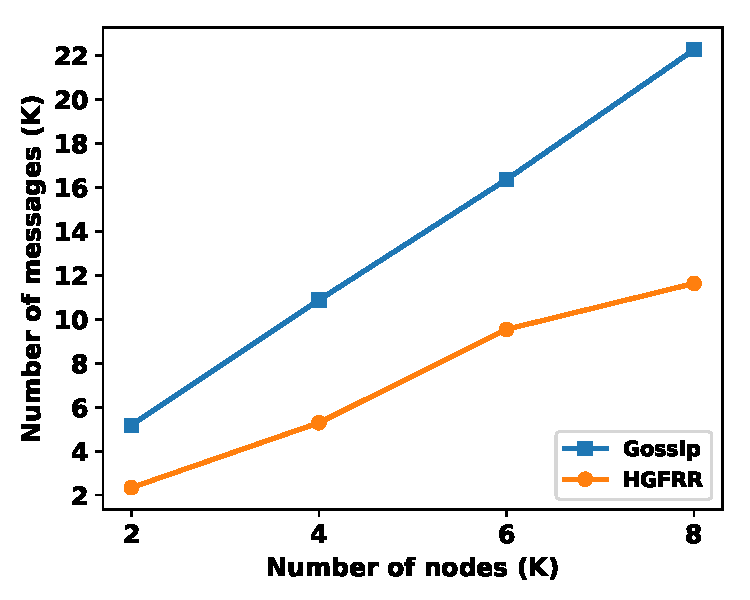
\includegraphics[width=\textwidth]{figures/hgfr_ourgossip_num_msg_on_num_node.pdf}
    \caption{Message complexity with respect to number of nodes.}
    \label{hgfr_ourgossip_num_msg_on_num_node}
    \end{subfigure}
    ~
    \begin{subfigure}[b]{0.23\textwidth}
	  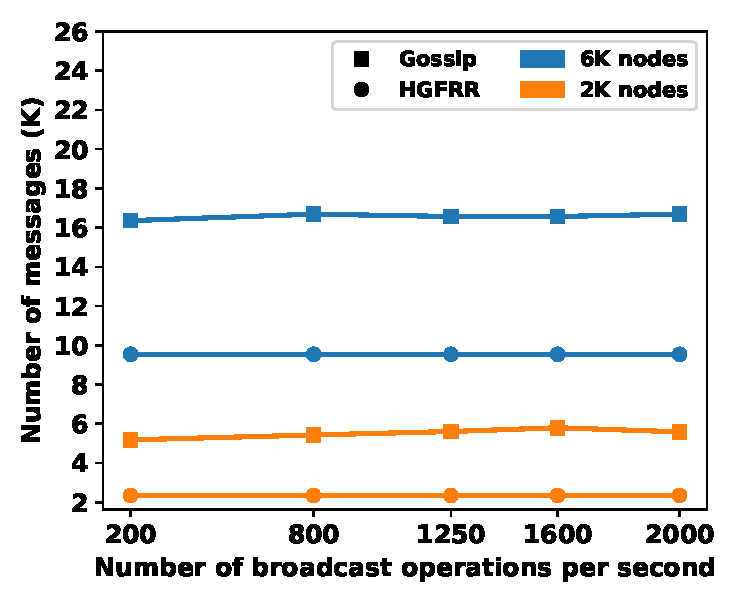
\includegraphics[width=\textwidth]{figures/hgfr_ourgossip_num_msg_on_tps.pdf}
	  \caption{Message complexity with respect to rate of broadcast operations.}
    \label{hgfr_ourgossip_num_msg_on_tps}
    \end{subfigure}

	\caption{Comparison of message complexity between Kademlia-based Gossip and \xxx.}
	\label{fig_hgfr_ourgossip_msg}
	\vspace{-0.5cm}
\end{figure}
  

talk about the performance improvement in terms of convergence time, message complexity.

\subsubsection{Broadcast}

\begin{figure*}[t]
  \centering
    \begin{subfigure}[t]{0.35\textwidth}
	  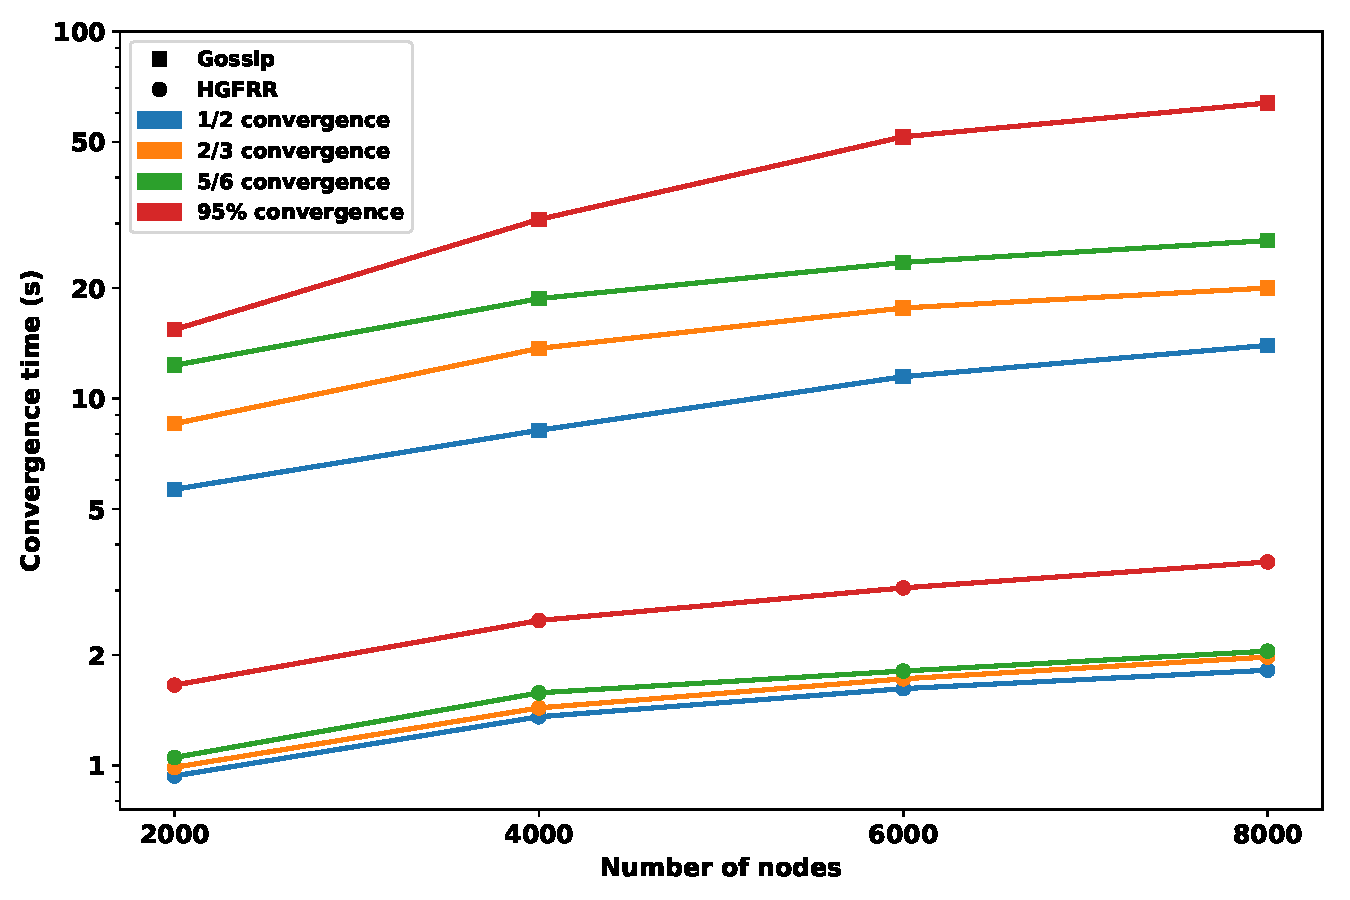
\includegraphics[width=\textwidth]{figures/hgfr_ourgossip_cvgtime_on_num_nodes.pdf}
	  \caption{Convergence time with respect to number of nodes.}
	  \label{hgfr_ourgossip_cvgtime_on_num_nodes}
    \end{subfigure}
	~
    \begin{subfigure}[t]{0.3\textwidth}
    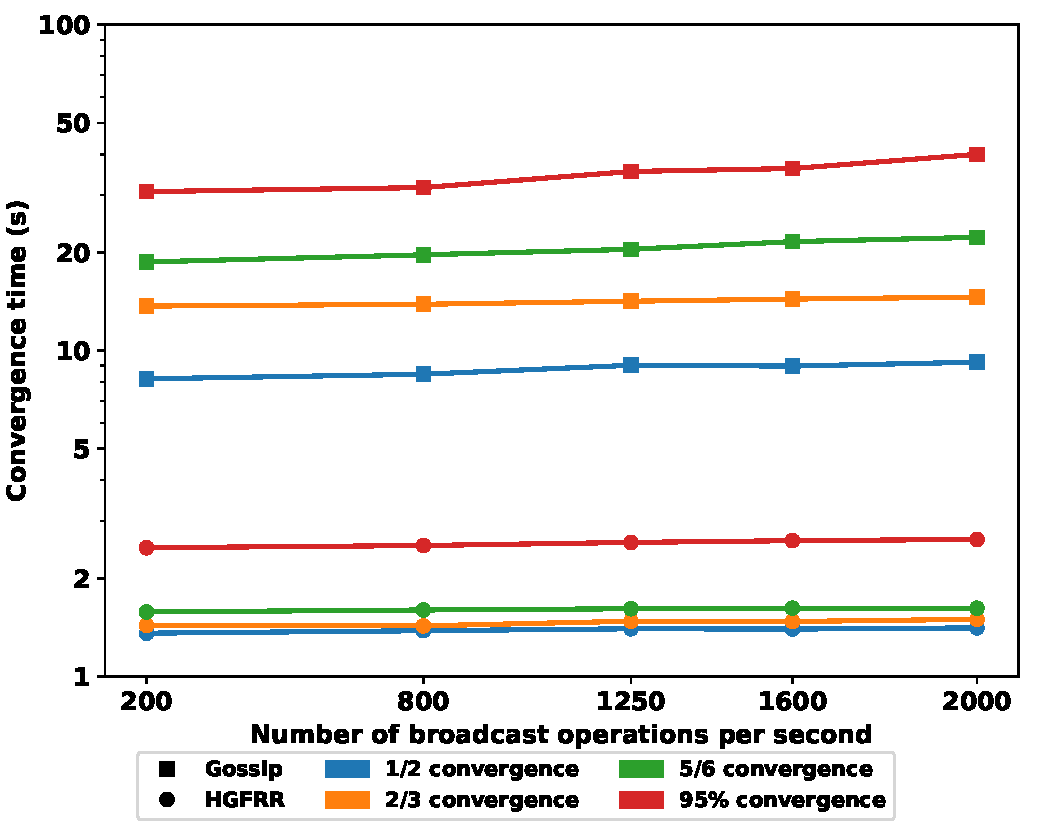
\includegraphics[width=\textwidth]{figures/hgfr_ourgossip_cvgtime_on_tps_2k.pdf}
    \caption{Convergence time with respect to broadcast rate under 2K nodes.}
    \label{hgfr_ourgossip_cvgtime_on_tps_2k}
    \end{subfigure}
    ~
    \begin{subfigure}[t]{0.3\textwidth}
	  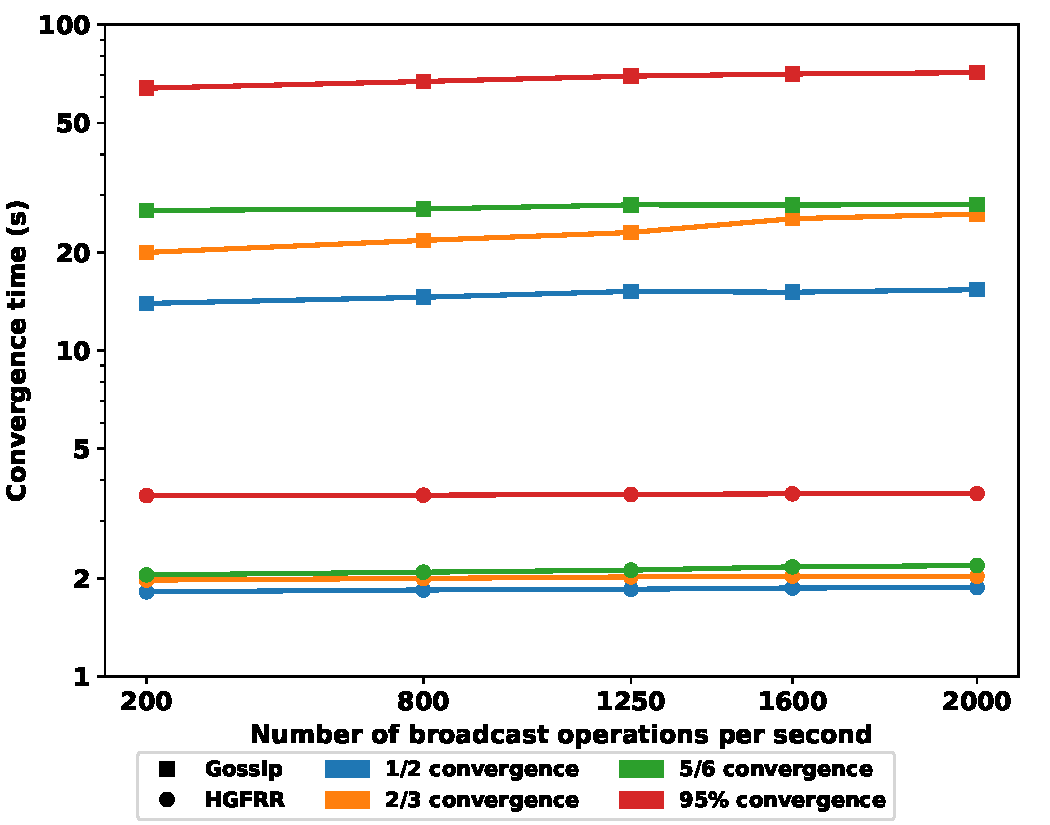
\includegraphics[width=\textwidth]{figures/hgfr_ourgossip_cvgtime_on_tps_6k.pdf}
	  \caption{Convergence time with respect to broadcast rate under 6K nodes.}
    \label{hgfr_ourgossip_cvgtime_on_tps_6k}
    \end{subfigure}

	\caption{Comparison of convergence time between Kademlia-based Gossip and \xxx.}
	\label{fig_eth_ourgossip_cvgtime}
	\vspace{-0.5cm}
\end{figure*}

\subsection{Fault tolerance}
\begin{figure}[ht]
	\centering
	  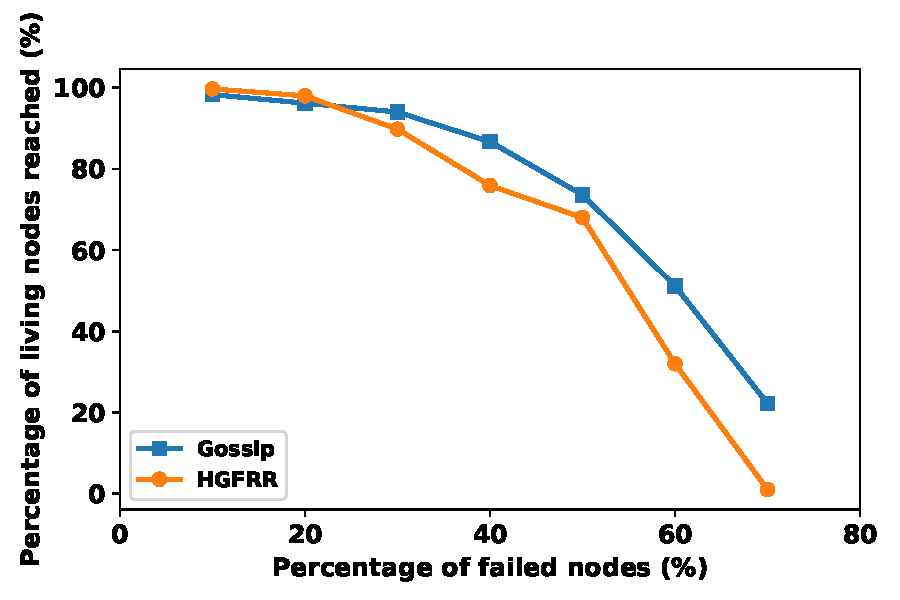
\includegraphics[width=0.46\textwidth]{figures/hgfr_ourgossip_fault.pdf}

	  \caption{Fault tolerance of \xxx and Gossip.}
	  \label{fig_hgfr_gossip_ft}
	  \vspace{-0.5cm}
  \end{figure}

\subsection{End-to-end comparison}

\begin{figure}[ht]
  \centering
    \begin{subfigure}[b]{0.23\textwidth}
    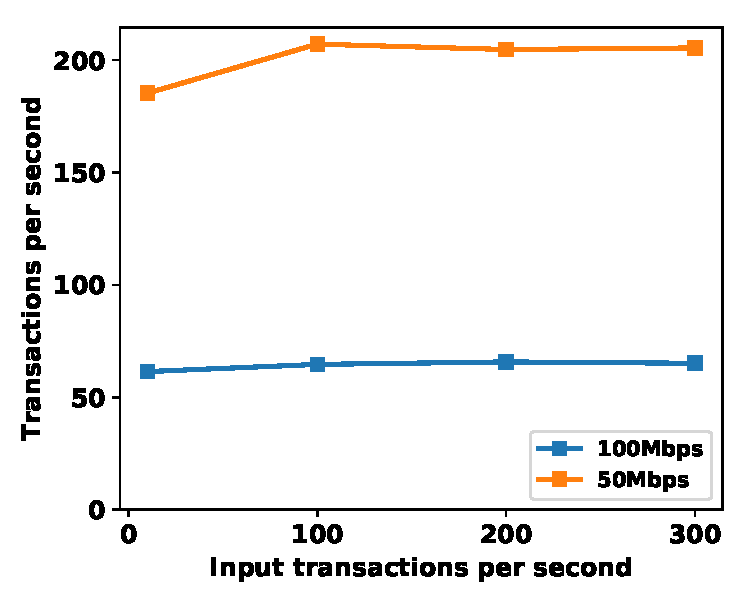
\includegraphics[width=\textwidth]{figures/eos_hgfr_e2e_tps_on_input.pdf}
    \caption{End-to-end performance of EOS transactions.}
    \label{eos_hgfr_e2e_tps_on_input}
    \end{subfigure}
    ~
    \begin{subfigure}[b]{0.23\textwidth}
	  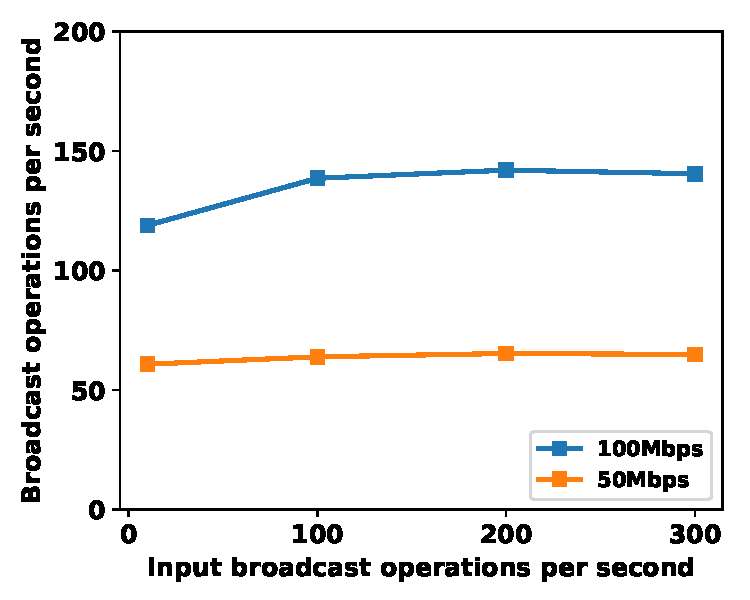
\includegraphics[width=\textwidth]{figures/eos_hgfr_micro_tps_on_input.pdf}
	  \caption{Broadcast performace of \xxx and the network of EOS.}
    \label{eos_hgfr_micro_tps_on_input}
    \end{subfigure}

	\caption{Comparison betweem EOS and \xxx.}
	\label{fig_eos_hgfr}
	\vspace{-0.5cm}
\end{figure}
  

\subsection{Security}

We uses WireShark \cite{chappell2010wireshark} to watch the packet sending out from a node and heading to the node. We counts three types of packets: around 17 kb, around 200 bytes, and less than 150 bytes, since they represents three types of messages correspondingly, i.e. the block, the transaction, and other messages including control messages or membership messages. We found that during one service term of a contact node, contact nodes of a ring cannot be differentiated from the normal nodes. By watching and recording for a long time, we found that the overall packet statistics show that all nodes have same percentages of sent and received three types of messages (See Table \ref{tab:packet1} and Table \ref{tab:packet2}). Therefore, due to the short service term of contact nodes and the similar percentages of all types of messages, it is hard for an outsider of the system to differentiate contact nodes from normal nodes.

\begin{table}
	\begin{tabular}{l*{6}{c}r}
		Node Type & $\sim17 KB$ & $\sim200 B$ & $<150 B$ \\
		\hline		
		Normal node in one term & 33.10\%	& 58.60\% & 5.90\% \\
		Contact node in one term & 34.00\%	& 61.20\% &4.50\%  \\
		Node at all time  & 33.70\%	& 60.90\% &4.60\%  \\
	\end{tabular}
	\caption{Send-Packet Analysis of Node in \xxx}
	\label{tab:packet1}
	\vspace{2mm}
	\begin{tabular}{l*{6}{c}r}
		Node Type & $\sim17 KB$ & $\sim200 B$ & $<150 B$ \\
		\hline		
		Normal node in one term & 35.50\% & 58.60\% & 5.60\% \\
		Contact node in one term & 34.40\% & 59.20\% & 4.70\%  \\
		Node at all time  & 34.60\% & 59.10\% & 5.10\%  \\
	\end{tabular}
	\caption{Receive-Packet Analysis of Node in \xxx}
	\label{tab:packet2}
\end{table}